\chapter{Технологическая часть}

В данном разделе описаны средства реализации, диаграмма классов, а так же интерфейс ПО. Так же представлены реализованные алгоритмы, которые были выбраны ранее.

\section{Средства реализации}
Для реализации программного обеспечения был выбран язык C\# по следующим причинам:
\begin{enumerate}
	\item Он поддерживает объектно-ориентированный стиль программирования;
	\item Личный опыт разработки на данном языке позволяет эффективно решать поставленные задачи;
	\item Язык обладает высокой производительностью, что важно при трассировке лучей и выполнении вычислений на процессоре.
\end{enumerate}

В качестве среды разработки был выбран Visual Studio, поскольку она достаточно удобна и обладает всем необходимым функционалом для реализации поставленной задачи. В частности, использование библиотеки WPF позволяет реализовать современный и функциональный пользовательский интерфейс, а средства Visual Studio упрощают разработку этого интерфейса.

\section{Диаграмма классов}
На рисунке ниже представлена UML-диаграмма классов. Она отображает структуру и взаимосвязи между  классами, что позволяет наглядно представить архитектуру программного обеспечения и взаимодействие его компонентов.

\begin{table}[H]
	\centering
	\begin{tabular}{p{1\linewidth}}
		\centering
		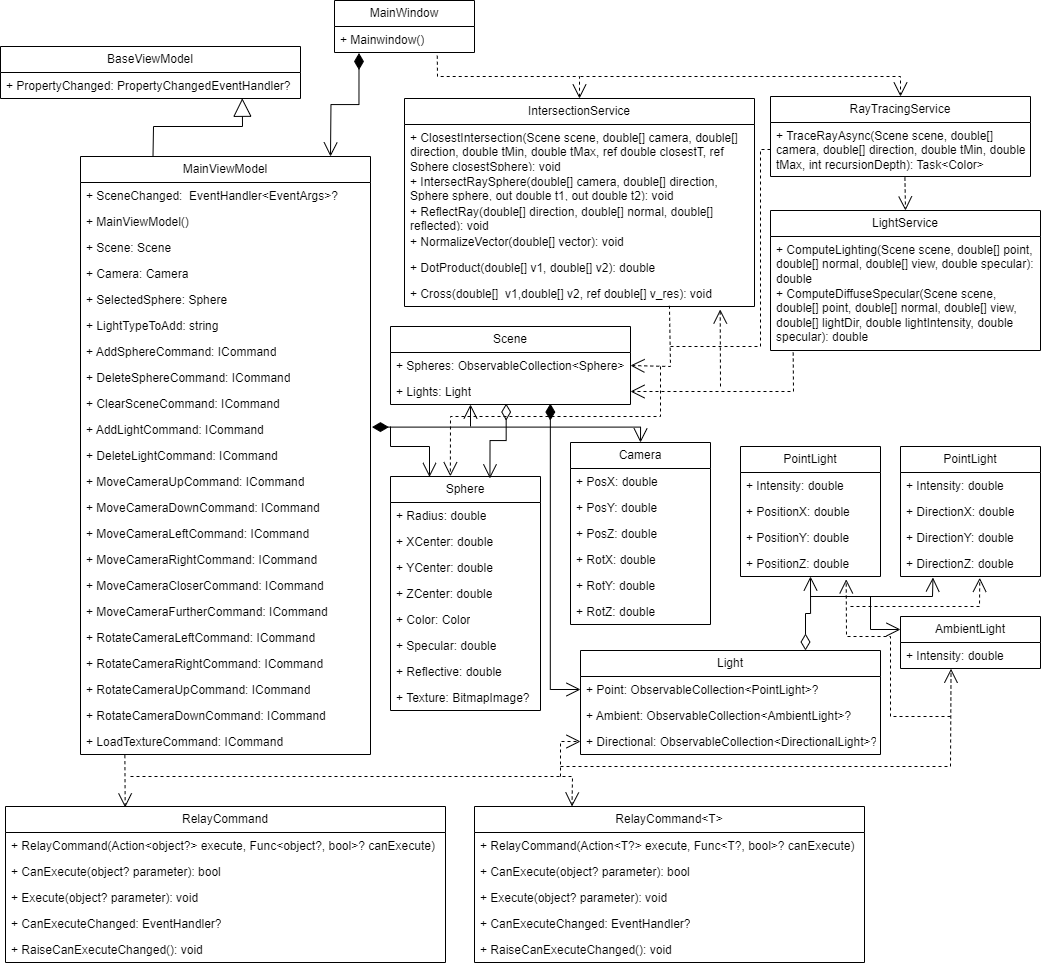
\includegraphics[width=1.0\linewidth]{include/3-1.drawio.png}
		\captionof{figure}{UML-диаграмма}
		\label{img:3-1}
	\end{tabular}
\end{table}

\section{Реализация алгоритмов}

Для начала рассмотрим реализацию вспомогательных функций.
\begin{lstlisting}[caption={Реализация вспомогательных функций для обработки векторов: отражение луча, нормализация вектора, вычисление скалярного произведения и векторного произведения.}, label={lst:3-1}]
public static void ReflectRay(double[] direction, double[] normal, double[] reflected)
{
	double dotProduct = DotProduct(direction, normal);
	reflected[0] = 2 * normal[0] * dotProduct - direction[0];
	reflected[1] = 2 * normal[1] * dotProduct - direction[1];
	reflected[2] = 2 * normal[2] * dotProduct - direction[2];
}

public static void NormalizeVector(double[] vector)
{
	double length = Math.Sqrt(vector[0] * vector[0] + vector[1] * vector[1] + vector[2] * vector[2]);
	if (length > 1e-6)
	{
		vector[0] /= length;
		vector[1] /= length;
		vector[2] /= length;
	}
}
public static double DotProduct(double[] v1, double[] v2)
{
	return v1[0] * v2[0] + v1[1] * v2[1] + v1[2] * v2[2];
}

public static void Cross(double[]  v1,double[] v2, ref double[] v_res)
{
	v_res[0] = v1[1] * v2[2] - v1[2] * v2[1];
	v_res[1] = v1[2] * v2[0] - v1[0] * v2[2];
	v_res[2] = v1[0] * v2[1] - v1[1] * v2[0];
}
\end{lstlisting}

Теперь рассмотрим функции, вычисляющие пересечения лучей и сфер.
\begin{lstlisting}[caption={Функции для нахождения ближайшего пересечения луча с какой-либо сферой на сцене.}, label={lst:3-2}]
public static void ClosestIntersection(Scene scene, double[] camera, double[] direction, double tMin, double tMax, ref double closestT, ref Sphere closestSphere)
{
	foreach (var sphere in scene.Spheres)
	{
		double t1, t2;
		IntersectRaySphere(camera, direction, sphere, out t1, out t2);
		if (tMin <= t1 && t1 <= tMax && t1 < closestT)
		{
			closestT = t1;
			closestSphere = sphere;
		}
		if (tMin <= t2 && t2 <= tMax && t2 < closestT)
		{
			closestT = t2;
			closestSphere = sphere;
		}
	}
}

public static void IntersectRaySphere(double[] camera, double[] direction, Sphere sphere, out double t1, out double t2)
{
	double r = sphere.Radius;
	double cx = camera[0] - sphere.XCenter;
	double cy = camera[1] - sphere.YCenter;
	double cz = camera[2] - sphere.ZCenter;
	
	double a = direction[0] * direction[0] + direction[1] * direction[1] + direction[2] * direction[2];
	double b = 2 * (cx * direction[0] + cy * direction[1] + cz * direction[2]);
	double c = cx * cx + cy * cy + cz * cz - r * r;
	
	double discriminant = b * b - 4 * a * c;
	
	
	if (discriminant < 0)
	{
		t1 = double.PositiveInfinity;
		t2 = double.PositiveInfinity;
	}
	else
	{
		double sqrtDiscriminant = Math.Sqrt(discriminant);
		if (double.IsNaN(sqrtDiscriminant))
		{
			t1 = double.PositiveInfinity;
			t2 = double.PositiveInfinity;
		}
		else
		{
			t1 = (-b - sqrtDiscriminant) / (2.0 * a);
			t2 = (-b + sqrtDiscriminant) / (2.0 * a);
		}
	}
}
\end{lstlisting}

Так же необходимо учесть влияние света.
\begin{lstlisting}[caption={Функции для вычисления освещения в сцене.}, label={lst:3-3}]
public static double ComputeLighting(Scene scene, double[] point, double[] normal, double[] view, double specular)
{
	double intensity = 0;
	
	foreach (var ambient in scene.Lights.Ambient)
	intensity += ambient.Intensity;
	
	foreach (var pointLight in scene.Lights.Point)
	{
		double[] lightDir = { pointLight.PositionX - point[0], pointLight.PositionY - point[1], pointLight.PositionZ - point[2] };
		IntersectionService.NormalizeVector(lightDir);
		intensity += ComputeDiffuseSpecular(scene, point, normal, view, lightDir, pointLight.Intensity, specular);
	}
	
	foreach (var directional in scene.Lights.Directional)
	{
		double[] lightDir = { directional.DirectionX, directional.DirectionY, directional.DirectionZ };
		IntersectionService.NormalizeVector(lightDir);
		intensity += ComputeDiffuseSpecular(scene, point, normal, view, lightDir, directional.Intensity, specular);
	}
	
	return intensity;
}

private static double ComputeDiffuseSpecular(Scene scene, double[] point, double[] normal, double[] view, double[] lightDir, double lightIntensity, double specular)
{
	double diffuseIntensity = IntersectionService.DotProduct(normal, lightDir) * lightIntensity;
	if (diffuseIntensity < 0) diffuseIntensity = 0;
	
	double specularIntensity = 0;
	if (specular >= 0)
	{
		double[] reflectDir = new double[3];
		IntersectionService.ReflectRay(lightDir, normal, reflectDir);
		double spec = IntersectionService.DotProduct(reflectDir, view);
		if (spec > 0)
		{
			specularIntensity = Math.Pow(spec, specular) * lightIntensity;
		}
	}
	return Math.Max(0, Math.Min(1, diffuseIntensity + specularIntensity));
}
\end{lstlisting}

Перед отображением пикселей нужно учитывать отражаемость объектов и интентивность цветов.
\begin{lstlisting}[caption={Функции для корректировки интенсивности цвета и расчета отраженного цвета.}, label={lst:3-4}]
private static Color AdjustIntensity(Color color, double intensity)
{
	byte r = (byte)Math.Min(255, Math.Max(0, color.R * intensity));
	byte g = (byte)Math.Min(255, Math.Max(0, color.G * intensity));
	byte b = (byte)Math.Min(255, Math.Max(0, color.B * intensity));
	return Color.FromRgb(r, g, b);
}

private static Color AdjustReflection(Color localColor, Color reflectionColor, double reflectivity)
{
	byte r = (byte)Math.Min(255, Math.Max(0, localColor.R * (1 - reflectivity) + reflectionColor.R * reflectivity));
	byte g = (byte)Math.Min(255, Math.Max(0, localColor.G * (1 - reflectivity) + reflectionColor.G * reflectivity));
	byte b = (byte)Math.Min(255, Math.Max(0, localColor.B * (1 - reflectivity) + reflectionColor.B * reflectivity));
	return Color.FromRgb(r, g, b);
}
\end{lstlisting}

Остается наложитить текстурные карты на поверхность сфер.

\begin{lstlisting}[caption={Учет текстуры на поверхности сфер.}, label={lst:3-5}]
private static async Task<Color> GetColorFromTextureAsync(Sphere sphere, double[] normal)
{
	double u = 0;
	double v = 0;
	
	ComputeTextureCoordinates(normal, ref u, ref v);
	
	int x = (int)(u * sphere.Texture?.PixelWidth??0);
	int y = (int)(v * sphere.Texture?.PixelHeight??0);
	
	var pixels = new byte[4];
	
	await Application.Current.Dispatcher.InvokeAsync(() =>
	{
		sphere.Texture?.CopyPixels(new Int32Rect(x, y, 1, 1), pixels, 4, 0);
	});
	
	return Color.FromArgb(pixels[3], pixels[2], pixels[1], pixels[0]);
}

private static void ComputeTextureCoordinates(double[] normal, ref double u, ref double v)
{
	double phi = Math.Atan2(normal[1], normal[0]);
	double theta = Math.Acos(normal[2]);
	
	u = (phi + Math.PI) / (2.0 * Math.PI);
	v = theta / Math.PI;
}

private static double[] AdjustNormalWithTexture(BitmapSource texture, double[] normal, Color textureColor)
{
	double Bu = textureColor.R / 255.0;
	double Bv = textureColor.G / 255.0;
	double[] Nb = { Bu, Bv, 1 };
	IntersectionService.NormalizeVector(Nb);
	
	double[] T = new double[3];
	IntersectionService.Cross(normal, Nb, ref T);
	IntersectionService.NormalizeVector(T);
	
	double[] B = new double[3];
	IntersectionService.Cross(normal, T, ref B);
	IntersectionService.NormalizeVector(B);
	
	double[] Nt = { IntersectionService.DotProduct(T, Nb), IntersectionService.DotProduct(B, Nb), IntersectionService.DotProduct(normal, Nb) };
	return new double[] { normal[0] + Nt[0], normal[1] + Nt[1], normal[2] + Nt[2] };
}
\end{lstlisting}

В итоге реализовываем трассировку луча.
\begin{lstlisting}[caption={Трассировка луча.}, label={lst:3-6}]
public static async Task<Color> TraceRayAsync(Scene scene, double[] camera, double[] direction, double tMin, double tMax, int recursionDepth)
{
	double closestT = double.PositiveInfinity;
	Sphere? closestSphere = null;
	IntersectionService.ClosestIntersection(scene, camera, direction, tMin, tMax, ref closestT, ref closestSphere);
	if (closestSphere == null)
	{
		return Colors.LightGray;
	}
	
	double[] intersectionPoint = { camera[0] + closestT * direction[0], camera[1] + closestT * direction[1], camera[2] + closestT * direction[2] };
	double[] normal = { intersectionPoint[0] - closestSphere.XCenter, intersectionPoint[1] - closestSphere.YCenter, intersectionPoint[2] - closestSphere.ZCenter };
	IntersectionService.NormalizeVector(normal);
	
	if (closestSphere.Texture != null)
	{
		Color textureColor = await GetColorFromTextureAsync(closestSphere, normal);
		normal = AdjustNormalWithTexture(closestSphere.Texture, normal, textureColor);
		IntersectionService.NormalizeVector(normal);
	}
	
	double[] viewDirection = { -direction[0], -direction[1], -direction[2] };
	double intensity = LightService.ComputeLighting(scene, intersectionPoint, normal, viewDirection, closestSphere.Specular);
	Color localColor = AdjustIntensity(closestSphere.Color, intensity);
	
	double reflectivity = closestSphere.Reflective;
	if (recursionDepth <= 0 || reflectivity <= 0)
	{
		return localColor;
	}
	
	double[] reflectionDirection = new double[3];
	IntersectionService.ReflectRay(viewDirection, normal, reflectionDirection);
	
	Color reflectionColor = await TraceRayAsync(scene, intersectionPoint, reflectionDirection, 0.001, double.PositiveInfinity, recursionDepth - 1);
	Color finalColor = AdjustReflection(localColor, reflectionColor, reflectivity);
	
	return finalColor;
}
\end{lstlisting}

Для ускорения работы программы методы трассировки был реализованы асинхронными, поскольку алгоритм позволяет производить вычисления для каждого из лучей не зависимо от предыдущих и последующих результатов. Это очень сильно ускоряет работу программы и позволяет сделать интерфейс более отзывчивым, а работу в программе более приятной для пользователя.

\section{Интерфейс программного обеспечения}

На рисунке \ref{img:3-2} представлен интерфейс программы.

\begin{table}[H]
	\centering
	\begin{tabular}{p{1\linewidth}}
		\centering
		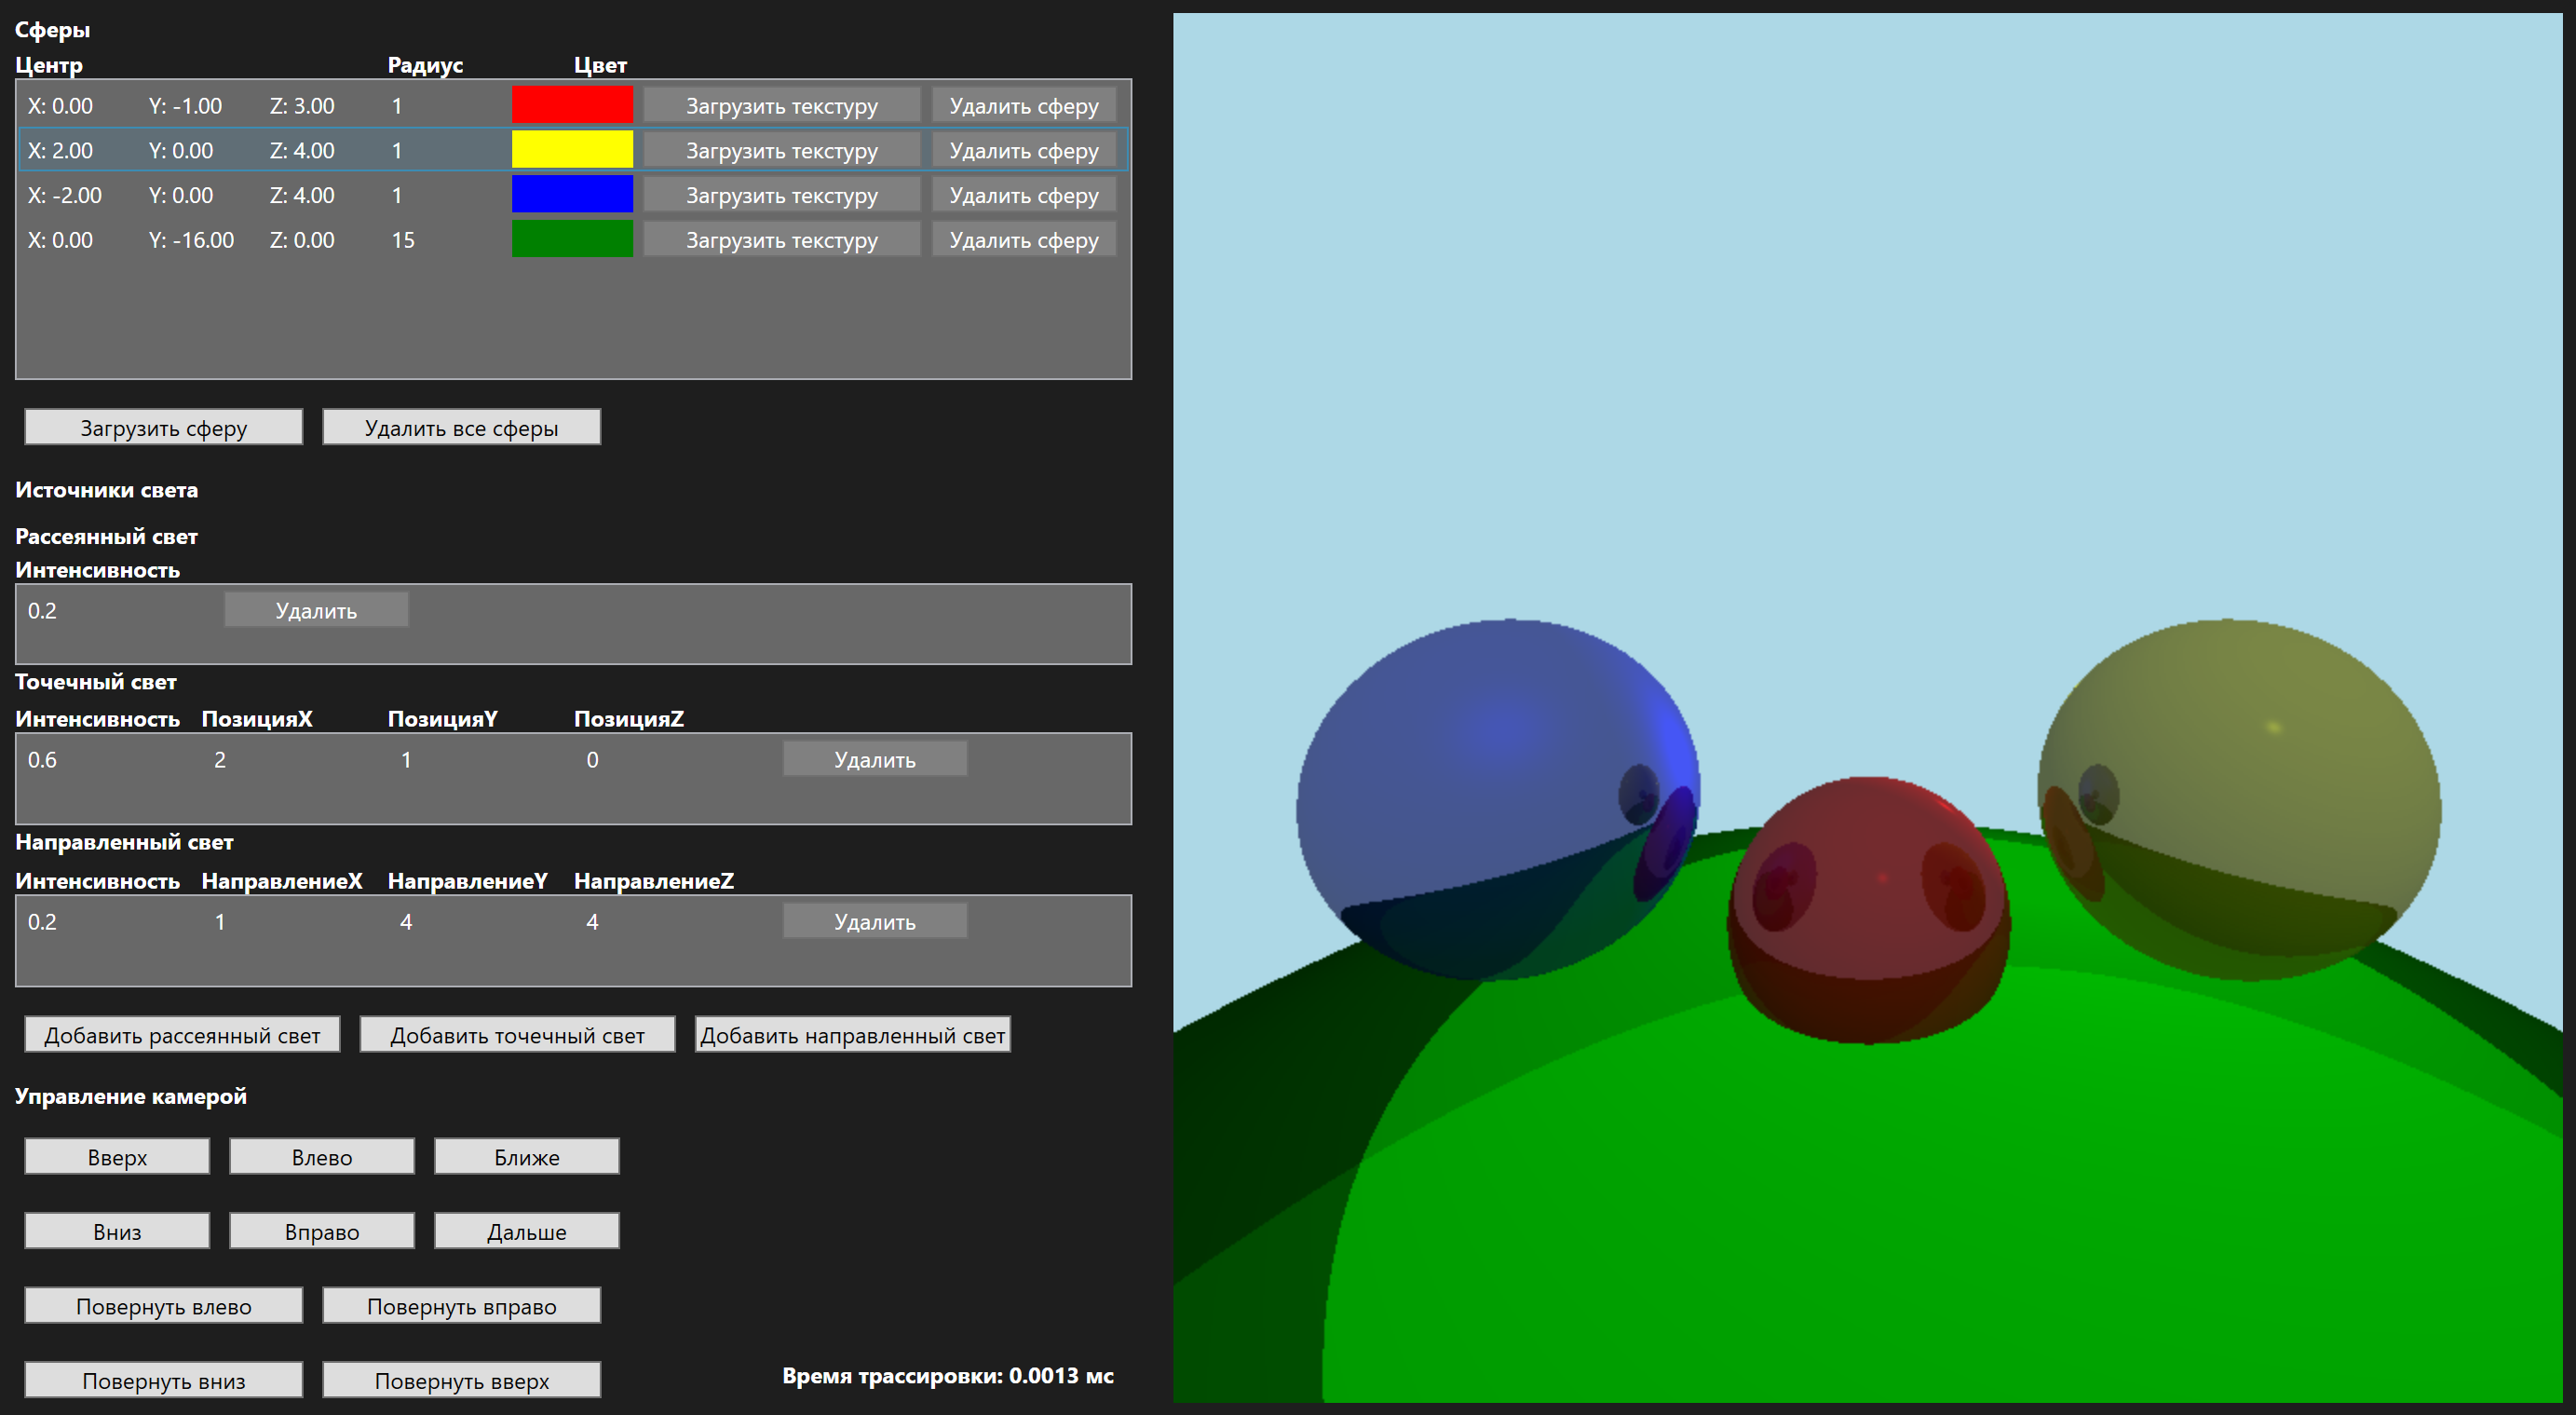
\includegraphics[width=1.0\linewidth]{include/3-2.png}
		\captionof{figure}{Интерфейс ПО}
		\label{img:3-2}
	\end{tabular}
\end{table}

В левой часте экрана расположены списки всех сфер на сцене и света на сцене, а так же различные кнопки: добавления и удаления сфер, добавления текстур на сферу, перемещения и вращения камеры, добавления и удаления света.

\section*{Вывод}
В этом разделе были выбраны средства реализации программы и составлена диаграмма классов, представлена реализация алгоритмов и пользовательский интерфейс.
